\section{Preface} \label{sec:preface}

\begin{figure}[htbp]
		\centering
		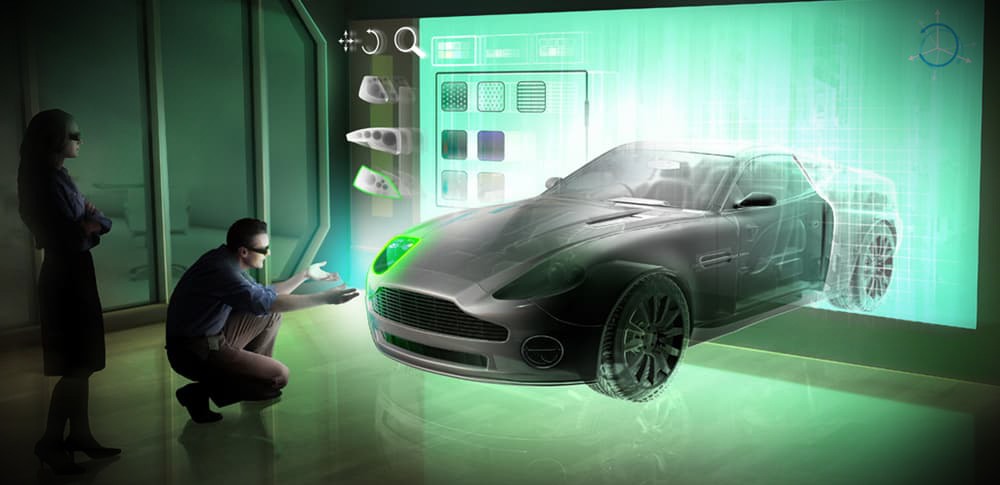
\includegraphics[width=1.0\textwidth]{figures/nvidia-3d-vision-pro}
		\caption[Promotional image for the NVIDIA 3D Vision Pro technology]{Promotional image for the \textit{NVIDIA 3D Vision Pro} technology (\textit{source:} \cite{Gizmag.2010}).}
		\label{fig:3dVisionary}
\end{figure}

Since the early years of science fiction story telling in books and movies, the concept of enriching our environment with digital information and other virtual content fascinates humanity. Movie franchises like \textit{Star Trek} and \textit{Star Wars} introduced unbelievable technology to a broad audience. First and foremost stories of space travel via huge ships with the help of fantastic inventions are meant to be entertaining. Having said that, the writers try to put the sci-fi technology into the context of a possible future science to make the shows more believable and exciting. The \textit{Holodeck}\index{Holodeck} in Star Trek is a good example of such an attempt. The Holodeck is an  environment simulator, which creates virtual worlds with the help of holographic projections in special rooms. It is used by the crew of the Enterprise for entertainment but also for training purposes. Although we can not yet imagine how to create a holographic image with which we can interact in such a way, the idea of fully accessable virtual worlds, the \textit{virtual reality} (see \autoref{sec:VAR})\footnote{The Holodeck may fall into the category of either a VR or an AR environment. The projection creates virtual content and the users can fully interact with it. The Holodeck itself is just a blank room, which makes the people interacting with it the only \enquote{real components}. Therefore there is no virtual overlayed \enquote{real} environment but only the virtual world the users have access to. According to the definitions used in this thesis (\autoref{sec:VAR}), the Holodeck is more of a VR application.}, has been a heavily researched field since the mid 19th century (compare with \cite{Nasa.2009}, \cite[p.3]{Toennis.2010}, \cite[p.19 et seq.]{Doerner.2013} and \cite[p.4 et seq.]{Burdea.2003}).

However, in many ways the actual development of the required hardware and software is still in its early stages (see \autoref{sec:history} for a historical overview of this topic), and although the concept was promising, we spent too many years \enquote{trapped} in the second dimension, leading to disappointments and the loss of people's confidence in the technology.

But with the improvement of sensors, graphics computation and displays the development of AR and VR applications can finally make significant progress. While the entertainment industry seems to be the most anticipated and closely followed development by the general public, the research on \textit{computer vision}\footnote{An explanation on this topic can be found at \autoref{ssec:cv}.} is still mostly driven by the military, NASA, the medical field and other technical industries. The tracking, recognition, analyzation, and finally digitization of real world objects and persons are important research fields for 3-D computer vision. In the future, surgeries will be fully supported with an AR overlay which displays the insides of the patient in real-time\footnote{The technology, with which the surgeons can see in real-time stereo vision with the help of tracking markers and stereoscopic glasses, is already far advanced (see \cite{Lowe.2016} for more examples).} and military drones could be able to distinguish between civilian and military buildings. Autonomous cars will reduce the risks on the streets and customers could design their individualized products interactively (see \autoref{fig:3dVisionary} for the vision NVIDIA presented in their promotional image for their new 3-D technology).

Despite all the recent successes, researchers are still struggling to reconstruct 3-D shapes and analyze/ interpret images in their entirety. But why is it so difficult? Why are people still disappointed? This misperception can be dated back to the early stages of robotics and artificial intelligence, in which it was initially believed that computer vision would be the easiest step to achieve (\cite[p.5]{Szeliski.2011}). 

Richard Szeliski, author of \textit{Computer Vision - Algorithms and Applications}, calls it an \enquote{inverse problem}: we try to find a solution on a basis of insufficient information provided by our imperfect technologies. We must turn to a physics- and mathematics-based approach to fill in these missing gaps and to create better \textit{models} of our real world. These include, for example, the modeling of shading and light reflection or the computation of the natural movement of colliding objects (compare with \cite[p.3 et seqq.]{Szeliski.2011}).  

In conclusion, the problems with computer vision can be broken down to mathematical algorithms, which are still merely models and subject to a multitude of errors. Some of these algorithms shall be the topics of this thesis.  
 
\begin{itemize}
\item computer vision 

\item optronis, highspeed cams --> why?
\end{itemize}
 
\section{About this thesis}
The present thesis is submitted in fulfillment of the requirements for the degree of Master of Science in \textit{Computer Science in Media} of the faculty of \textit{Digital Media}. The high-speed cameras and their software components as well as technical support were provided by the company \textit{Optronis}.

--> fragestellung, aufgabenstellung, zu erreichender grad, wieso highspeed (lack of data --> come back to inverse problm), optronis --> on consumer level \\
--> the goal for consumer market is to make all easy and cheap 
--> the goal for industry is to connect virtual and real world content seamlessly  

- could use ideal images - already a lot of studies --> not real

\textit{Optronis}\index{Optronis} is a German company which is specialized in the field of ultra-fast optical measuring systems since 1986\footnote{Check Optronis' webpage for more detailed information about the company and its products: \url{http://www.optronis.com}}. Their products are used for research and science in several fields. Both their high-speed cameras for precision measurements and their streak camera technology, which makes photons visible, help monitoring and analyzing processes that are otherwise invisible for the human eye (\cite{Optronis.2016}).

This thesis is loosely linked to my bachelor's thesis, in which the \textit{Oculus Rift}, a head-mounted display\footnote{More information about head-mounted displays can be found in \autoref{sec:VAR}. The  bachelor's thesis is digitally attached (in German).}, was transformed into an AR device with the help of two webcams. The software was developed in \CS and the shading language \textit{Cg} in the \textit{Unity Engine} (\cite{Haefele.2014}).     

\todo{--> zeitplan, --> vorgehensweise}


\begin{itemize}
\item Kapitelaufbau: hangelt sich an Pipeline lang - v.a. grundlagen und Implementierung
\item Background: basic definitions/ wording and historical background
\item related works: paper, matlab examples, theses
\item Math. principles: algos and calculations
\item Implementation: step by step, also includes some more math. principles that are more specific
\item closure: ...
\item glossar, why?
\end{itemize}

--> notation, see Szeliski p.25 for reference


\begin{figure}[htbp]
		\centering
		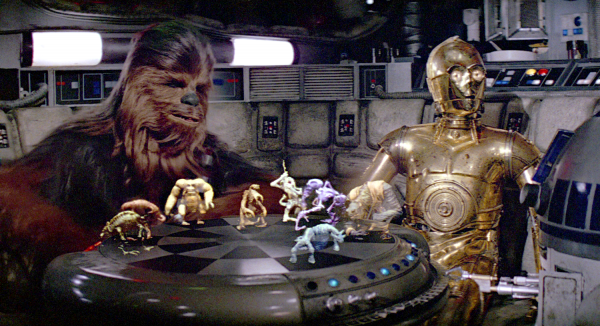
\includegraphics[width=0.8\textwidth]{figures/starWars}
		\caption[Bla]{Bla (\textit{source: 20th Century Fox ?} bla).}
		\label{fig:starWars}
\end{figure}
%\todo{another example for AR: star wars chess --> make two graphics with holodeck and star wars chess http://cdn.slashgear.com/wp-content/uploads/2014/06/falco-600x326.png }

